\newpage

\section{Metode og Proces}
I nedstående afsnit fremlægges metoder og processer brugt til udviklingen af
Dungeons and Gnoblins spillet kort, for at se mere om metode og proces henvises der til den vedhæftede process rapport.

\subsubsection{Projektforløb og møder}
Projektets endelige mål har været implementeringen af et text-based adventure game.
Hertil har gruppen gjort brug af agile develepment processen til at imødekomme dette mål.

Først har gruppen specifiseret Kravspecifikationerne for spillet, med ønsker om
hvilke features spillet har skulle inkludere.

I løbet af projektforløbet blev der afholdt to faste ugentlige møder. Et internt gruppemøde og et vejledemøde. Til hvert møde blev der gennemgået hvad der var blev arbejdet med, hvilke udfordringer der forekom samt hvad der fremadrettet skulle arbejdes med for hver af gruppens medlemmer. Dette gjorde vi i form af SCRUM for at give et bedre overblik for projektets fremgang og dermed vurderer om gruppen var bagud eller foran ift. Gruppens tidsplan.

\begin{figure}[H]
  \centering
  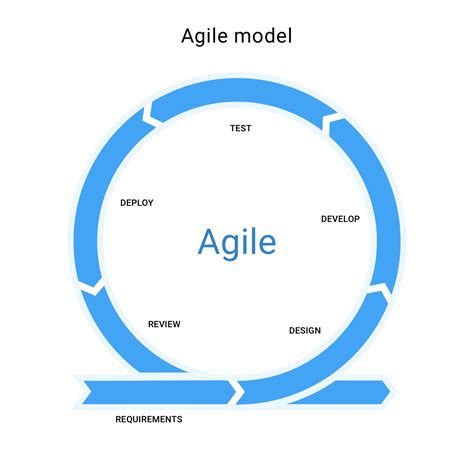
\includegraphics[scale=.5]{02-Body/Images/Agile.png}
  \caption{Viser et billed af agile modellen som består af mangle iterationer
           af design, develop, test, og deploy. Dette minder om continuous integration
           og har hindret mange problemmer for udviklingsforløbet}
  \label{fig:Agile}
\end{figure}

SCRUM og AGILE bringer klarhed til medlemmerne om deres roller og opgaver over en 
kommende tidperiode med en backlog over opgaver, som skal færdiggøres over et sprint (1 uge).
Ugentlige opdateringer og møder omkring potentielle problemmer udviklingsforløbet betyder
at gruppen har kunne tage hånd om evt. problemmer tidligt i forløbet og derved løse dem
før de har udviklet sig til større problemmer.
Til styring og implementering af souce code er der i gruppen blevet benyttet git som et versions styrings system.

\subsection{Modellering}
Projektet benytter UML til at beskrive og modellere software-- arkitektur
og design, hvilket gør det nemt at simplificere og visualisere strukturen på software
løsningen. 

Selve arkitekturen er vist med C4 modellen som giver et lageret indblik i både
akitekturen på et højt niveau, men med evnen til at give en detaljeret beskrivelse
af systemmets komponenter og deres kommunikation med hinanden.

\begin{figure}[H]
  \centering
  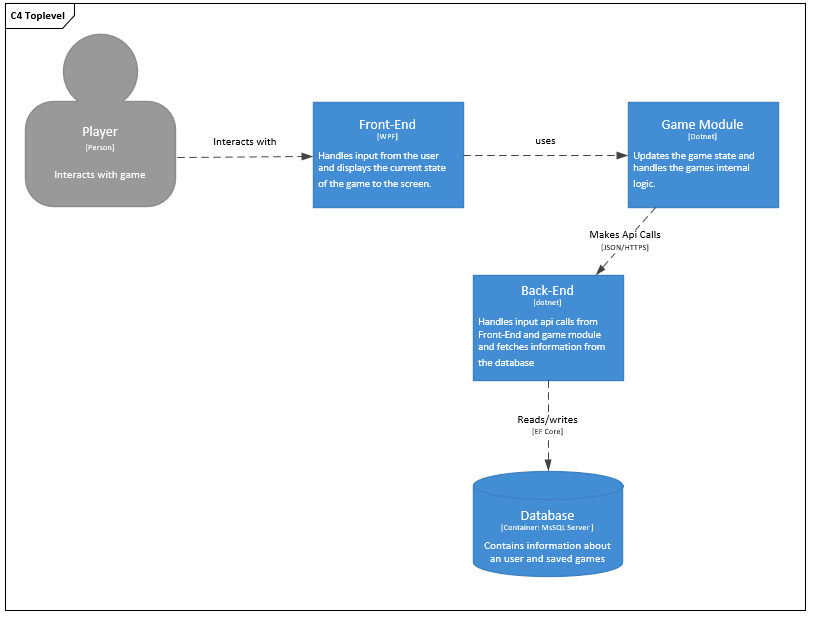
\includegraphics[scale=0.8]{02-Body/Images/C4TopLvlDB.PNG}
  \caption{Et eksempel på en C4 model, og det overblik et sådan diagram kan give over et system.}
  \label{fig:c4}
\end{figure}

STM og SD diagrammer er brugt til at give programmets udførsel struktur, og fungerer,
som en hjælp til at visualisere programmets forskellige states og flow of execution.
Det giver et nemt overblik over hvordan funktionskald mellem forskellige komponenter
har skal fungere således, at der ikke opstår misforsåelse grupperne imellem. 

Generelt er arkitekturen opbygget som "pseudo" diagrammer. Dvs. de ligner ikke fuldstændigt det endelige design, men har til formål at vise den overordnede tankegang i systemet og samtidig virke som et udviklingsværktøj til at videreudvikle systemet. Da der i gruppen er blevet arbejdet iterativt, er der forskelle mellem diagrammer for arkitektur og design,da der er blevet tilføjet flere moduler og funktioner undervejs. Den overordnede tanke i projektet er der dog ikke blevet ændret på.

\subsubsection{Iterativ Udviklingsforløb}

AGILE og continuous integration fungerer på en naturlig iterativ måde, der tillader 
ændringer til måde designet og implementeringen undervejs i udviklingsforløbet.
Under hvert SCRUM møde er der taget stilling til om, der skulle laves ændringer i 
gruppens tilgang til projektet, altså om en implementering skulle ændres. \\



